\begin{center}

  \begin{tabular}{rp{16cm}lp{20cm}}%{rl}

  % after \\: \hline or \cline{col1-col2} \cline{col3-col4} ...

  论文地址:& \href{https://openreview.net/pdf?id=rkem91rtDB}{https://openreview.net/pdf?id=rkem91rtDB} \\
  来源:& ICLR, 2020 \\
  作者:& Lichen Wang, Bo Zong, et al. \\
  源码:& \href{https://github.com/wenwen0319/SEED-Reimplementation}{SEED-Reimplementation} \\
  slides:& \href{https://github.com/wanglichenxj/Inductive-and-Unsupervised-Representation-Learning-on-Graph-Structured-Objects/blob/master/presentations/ICLR_slides.pdf}{{\footnotesize SEED}}\\
  关键词:& \textbf{unsupervised learning, graph representation} \\
  写于:& \date{2021-03-01}
  \end{tabular}
\end{center}

该论文\cite{SEED_Lichen}主要解决的是图结构数据的无监督的、inductive形式的表征问题。通常在无监督的图表征问题中,主要以重建损失为主导进行训练,但是在计算重建损失时通常要涉及到图的相似性计算,而图的相似性计算是一个十分复杂、耗时的过程,论文提出了一个通用的框架SEED(Sampling, Encoding and Embedding Distribution)用于无监督的学习图结构对象的表征。

\paragraph{问题定义}
目标很简单,给定一个graph,学习它的表征。

\paragraph{SEED思路}
\begin{figure}[h]
	\centering
	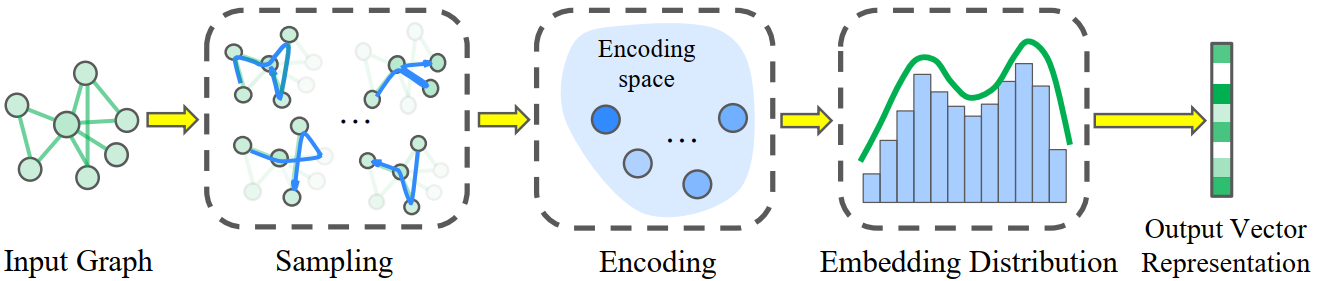
\includegraphics[width=.8\textwidth]{pics/SEED.png}
	\caption{SEED}
	\label{fig:seed}
\end{figure}
如Fig.\ref{fig:seed}所示,SEED主要分为三个部分:
\subparagraph{Sampling}
从输入的图中采样出多个子图。为了使得采样到的子图更具代表性,论文中提出了一种新的采样方法 --- WEAVE(random Walk with EArliest Visit timE)。该方法与通常的随机游走不一样,WEAVE是带结点访问时间戳的。
\begin{figure}[h]
	\centering
	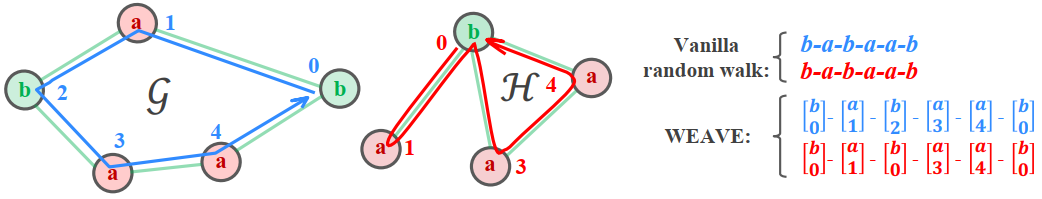
\includegraphics[width=.8\textwidth]{pics/WEAVE.png}
	\caption{WEAVE与随机游走对比}
	\label{fig:weave}
\end{figure}
如Fig.\ref{fig:weave}所示,WEAVE的区分能力比平凡的搜集游走更强。每一个WEAVE都代表一个采样到的子图,可以用一个矩阵表示:$X=\left[\mathbf{x}^{(0)}, \mathbf{x}^{(1)}, \cdots, \mathbf{x}^{(k)}\right]$,其中$\mathbf{x}^{(p)} = [\mathbf{x}_a^{(p)}, \mathbf{x}_t^{(p)}]$,$\mathbf{x}_a^{(p)}$表示在时间$p$时访问到的结点的特征,$\mathbf{x}_t^{(p)}$表示访问到该结点时的时间向量。\tbc{red}{注意,如果访问到了已经访问过的结点则$\mathbf{x}_t^{(p)}$为最早访问时的时间}。在论文中,$\mathbf{x}_t^{(p)}$采用one-hot编码。

\subparagraph{Encoding}
将每一个采样到的子图编码为向量。直觉上,如果子图的表征质量好,那么就能在子图表征地基础上较好地重建子图。论文中作者采样自编码器学习子图的表征,以重建损失作为损失函数。至此,$s$个子图$\{X_1, ..., X_s\}$被表示为$s$个向量$\{\mathbf{z}_1, ..., \mathbf{z}_s\}$。

\subparagraph{Embedding Distribution}
将上一阶段获得的多个子图的表征汇集作为输入图的表征。对于两个图,它们在表征空间中的距离应该与它们的子图向量分布距离类似,因此需要找到一个好的聚集函数来保留原先的子图表征分布距离,论文中采用的是$MMD$。
给定连个图$\mathcal{G}, \mathcal{H}$,子图表征分别为:$\{\mathbf{z}_1, ..., \mathbf{z}_s\}$和$\{\mathbf{h}_1, ..., \mathbf{h}_s\}$,则两者间的$MMD$为:
$$
\begin{aligned}
	\widehat{M M D}\left(P_{\mathcal{G}}, P_{\mathcal{H}}\right)=& \frac{1}{s(s-1)} \sum_{i=1}^{s} \sum_{j \neq i}^{s} k\left(\mathbf{z}_{i}, \mathbf{z}_{j}\right)+\frac{1}{s(s-1)} \sum_{i=1}^{s} \sum_{j \neq i}^{s} k\left(\mathbf{h}_{i}, \mathbf{h}_{j}\right) \\
	&-\frac{2}{s^{2}} \sum_{i=1}^{s} \sum_{j=1}^{s} k\left(\mathbf{z}_{i}, \mathbf{h}_{j}\right) \\
	=&\left\|\hat{\mu}_{\mathcal{G}}-\hat{\mu}_{\mathcal{H}}\right\|_{2}^{2}
\end{aligned}
$$
$\hat{\mu}_{\mathcal{G}}, \hat{\mu}_{\mathcal{H}}$分别表示两个图的kernel embedding,也就是最终的graph representation,分别定义为:
$$
\hat{\mu}_{\mathcal{G}}=\frac{1}{s} \sum_{i=1}^{s} \phi\left(\mathbf{z}_{i}\right), \quad \hat{\mu}_{\mathcal{H}}=\frac{1}{s} \sum_{i=1}^{s} \phi\left(\mathbf{h}_{i}\right)
$$
其中$\phi(\cdot)$是与核函数$k(\cdot, \cdot)$相关的特征映射函数(与SVM中的核技巧类似,将核函数的计算转化为更简单的计算形式)。
根据核函数的选择,$\phi(\cdot)$具有不同的形式,如RBF、MLP等。为了训练$\phi(\cdot)$,文中使用如下的近似误差,其中$\theta_m$为$\phi(\cdot)$的参数):
$$
J\left(\theta_{m}\right)=\left\|D\left(P_{\mathcal{G}}, P_{\mathcal{H}}\right)-\widehat{M M D}\left(P_{\mathcal{G}}, P_{\mathcal{H}}\right)\right\|_{2}^{2}
$$
通过最小化上述误差,就能学习到较好的聚集函数,在最终的表征中保留子图表征的分布距离。

该论文的方法与核方法有一定的相似性。论文还证明了同构的图的WEAVE的子图分布是类似的,并且对子图的采样长度进行了证明,详细内容可以参考论文。

\paragraph{方法解决的问题/优势}

\begin{itemize}

	\item 给出了无监督形式的、inductive的图结构对象表征学习方法
	\item 避免了复杂的图相似性计算,以类似于核技巧的方法较好地度量了图之间地距离
	\item 对相关地定理进行了证明

\end{itemize}



\paragraph{方法的局限性/未来方向}

\begin{itemize}

	\item 当图地规模较大时,采样的子图也会非常大,且可能需要采样地子图数量会很大

\end{itemize}